% =====================================================================
%  ch05_methodology_and_data.tex — Agent 3 (Python_Viz)
%  Numbers: comms/data_summary.json (single source of truth).
%  Scripts: build/scripts/ (run_all.py) · Figures: build/figures/
% =====================================================================
\chapter{מתודולוגיה ונתונים}
\label{ch:methodology}

\begin{managerbox}
מנהל סיכוני אשראי בבנק או סמנכ״ל כספים בחברה יזמית נדרש להעריך את חשיפתו לגל חדלות פירעון לפני התממשותו. פרק זה מתאר אילו נתונים אומתו, אילו הנחות נוספו ומדוע נבחרה סימולציה מכוילת. ההפרדה בין עובדה לתרחיש מאפשרת להחליף הנחה אחת ולראות כיצד משתנה המסקנה.
\end{managerbox}

\section{מקורות הנתונים ועיבודם}
\label{sec:ch5-sources}

המחקר נשען על נתוני בנק ישראל, הלמ״ס, משרד האוצר וה־\en{BIS}; נתון הזמין רק בדיווח משני מסומן ככזה (טבלה~\ref{tab:ch5-sources}).

\begin{table}[!htb]
\centering
\caption{מקורות הנתונים, תקופת הכיסוי ומעמד האימות}
\label{tab:ch5-sources}
\footnotesize
\begin{tabularx}{\tabmaxwidth}{>{\raggedleft\arraybackslash}p{3.2cm} R >{\centering\arraybackslash}p{2.0cm} >{\centering\arraybackslash}p{1.9cm}}
\toprule
\hd{סדרה} & \hd{מקור} & \hd{תקופה} & \hd{מעמד} \\
\midrule
ריבית בנק ישראל & החלטות הוועדה המוניטרית \cite{boi_rate_2026_09}; ריכוז משני \cite{boi_rate_decisions} & \en{2021–2026} & רשמי (\en{2026}) ומשני \\
מלאי דירות חדשות שלא נמכרו & נתוני הלמ״ס, דרך דיווח משני \cite{cbs_newdwellings,cbs_newdwellings_2026q3} & \en{2021–2026} & משני \\
עסקאות דירות & הכלכלן הראשי, דרך דיווח משני \cite{semerenko_market,toi_housing_2026_10} & \en{2021–2026} & משני \\
מדד מחירי הדירות & הלמ״ס \cite{cbs_priceindex_2026_222,toi_housing_2026_10} & \en{2021–2026} & שינויים שנתיים אומתו \\
חוב משקי בית לתוצר & \en{BIS} \cite{bis_hhdebt} & \en{2007}, \en{2025} & רשמי, מאומת \\
אשראי ליזמים וחשיפת בנקים & סקירת מערכת הבנקאות, בנק ישראל \cite{boi2026_recredit,boi2026_resloans} & \en{2024–2025} & רשמי, מאומת \\
הון, \en{RWA} ואשראי לבינוי ונדל״ן & דוחות רבעוניים של חמש הקבוצות (טבלה~\ref{tab:ch5-banks}) & \en{30.9.2026} & רשמי, מאומת \\
שיעור מבצעי המימון & הכלכלן הראשי \cite{mof_review_2026_08,nadlancenter_2026_08_promos} & \en{2026} & רשמי; לכיול \\
\bottomrule
\end{tabularx}
\end{table}

אומתו מול המקור (נכון ל־\en{16.11.2026}; נתוני הבנקים: \en{24.11.2026}) בעיקר נקודות של \en{2026}; ערכי \en{2021–2025} במלאי ובעסקאות ורמות מדד המחירים הם עוגנים משוחזרים, ומוצגים באיורים כקו ללא סמן.

\label{sec:ch5-cleaning}כל ערך הוזן לרישום נתונים יחיד עם תג מעמד: \en{official} (מאומת), \en{official\_\allowbreak approx} (רק חלק מהנקודות אומתו) או \en{calibrated} (פרמטר שקבע החוקר). עוגנים רבעוניים הומרו לסדרה חודשית באינטרפולציה לינארית, והריבית לסדרה מדרגתית לפי מועד כניסת כל החלטה לתוקף. מדד המחירים הוצג בבסיס ינואר \en{2021 = 100} (סעיף~\ref{sec:ch3-demand}). לעסקאות משמשת הגדרת הכלכלן הראשי \cite{toi_housing_2026_10}. ערך מאומת מוצג כעובדה עם מראה מקום; כל ערך אחר, ובכלל זה תוצאות הסימולציה, מוצג כ״תרחיש״, ״להמחשה״ או ״בהנחה כי״.

\section{חלופות מתודולוגיות ומטריצת החלטה}
\label{sec:ch5-alternatives}

שאלת המחקר משלבת השוואה לאחור של מנגנוני כשל והערכה צופה פני עתיד של עמידות המערכת ב״קיר המסירות״. נבחנו שלוש חלופות: \textbf{א — אקונומטריקה של סדרות עתיות}, מודל \term{וקטור אוטו־רגרסיבי}{VAR} או פאנל המקשרים ריבית, מחירים ומלאי לשיעורי כשל היסטוריים; \textbf{ב — סימולציה מבנית מכוילת}, מודלים מפורשים (\en{NPV}, זעזוע תשלום, \term{מונטה קרלו}{Monte Carlo} ורשת מבחני קיצון) המכוילים לנתונים רשמיים; ו\textbf{ג — חקר מקרים איכותני}, \term{מעקב תהליכים}{process tracing} ללא כימות. חמשת הקריטריונים והמשקלות נקבעו לפני שקלול הציונים, כדי למנוע התאמה בדיעבד. ציון כל קריטריון נע בין \en{1} ל־\en{5}, והציון המשוקלל של חלופה $j$ הוא

\begin{equation}
S_j=\sum_{i} w_i\, c_{ij}, \qquad \sum_i w_i = 1.0
\label{eq:ch5-score}
\end{equation}

כאשר $w_i$ הוא משקל הקריטריון ו־$c_{ij}$ ציון החלופה. טבלה~\ref{tab:ch5-matrix} מציגה את התוצאה.

\begin{table}[!htb]
\centering
\caption[מטריצת החלטה לבחירת השיטה]{מטריצת החלטה משוקללת לבחירת השיטה (משקלות נקבעו לפני הציונים)}
\label{tab:ch5-matrix}
\small
\begin{tabularx}{\tabmaxwidth}{R >{\centering\arraybackslash}p{1.2cm} >{\centering\arraybackslash}p{1.5cm} >{\centering\arraybackslash}p{1.5cm} >{\centering\arraybackslash}p{1.5cm}}
\toprule
\hd{קריטריון} & \hd{משקל} & \hd{א: \en{VAR}} & \hd{ב: סימולציה} & \hd{ג: איכותני} \\
\midrule
זמינות נתונים מתאימים & \en{0.30} & \en{2} & \en{4} & \en{5} \\
יכולת לענות על החלק הצופה פני עתיד & \en{0.25} & \en{2} & \en{5} & \en{3} \\
שקיפות ויכולת שחזור & \en{0.20} & \en{4} & \en{4} & \en{3} \\
עלות בזמן ובמשאבים & \en{0.15} & \en{3} & \en{4} & \en{5} \\
הפרדה בין עובדות להנחות & \en{0.10} & \en{4} & \en{4} & \en{2} \\
\midrule
\textbf{ציון משוקלל $S_j$} & \en{1.00} & \textbf{\en{2.75}} & \textbf{\en{4.25}} & \textbf{\en{3.80}} \\
\bottomrule
\end{tabularx}
\end{table}

חלופה ב זוכה בציון \en{4.25}. חלופה א נכשלת בהיעדר היסטוריה: מבצעי \en{20/80} התרחבו רק מ־\en{2023}, ומחזור המסירות הראשון טרם הניב סדרת כשלים לאמידה. חלופה ג אינה מייצרת מספרים שאפשר להעמיד מול ספי הרגולציה, ורכיביה האיכותניים משמשים בפרקים~\ref{ch:subprime} ו־\ref{ch:comparative}. היתרון של ב נשמר גם אם משקל ״זמינות נתונים״ עולה ל־\en{0.40} (\en{4.15} מול \en{4.00}).

\section{ארכיטקטורת הפתרון וזרימת הנתונים}
\label{sec:ch5-architecture}

איור~\ref{fig:ch5-architecture} מציג את זרימת הנתונים: רישום יחיד מזין חמישה מודלים, והרצת \en{\texttt{run\_all.py}} אחת משחזרת את כל האיורים והמספרים, עם זרע אקראי קבוע.

\begin{figure}[!htb]
\centering
\begin{english}
\scalebox{0.85}{%
\begin{tikzpicture}[font=\footnotesize\linespread{1}\selectfont,
  box/.style={rounded corners=2pt, align=center, minimum height=8mm},
  src/.style={box, draw=brandSteel, fill=brandPale, text width=2.4cm},
  mod/.style={box, draw=brandNavy, thick, fill=white, text width=2.5cm},
  sink/.style={box, draw=brandGreen, fill=brandGreen!8, text width=2.9cm},
  arr/.style={-{Stealth[length=2mm]}, brandSteel, thick}]
\node[src] (boi) at (0, 0)    {Bank of Israel\\rates, FSR};
\node[src] (cbs) at (0,-1.2)  {CBS\\inventory, prices};
\node[src] (mof) at (0,-2.4)  {MoF Chief Economist\\transactions};
\node[src] (bis) at (0,-3.6)  {BIS / FCIC /\\bank reports};
\node[mod, minimum height=4.4cm] (reg) at (3.7,-1.8) {\textbf{data\_sources.py}\\[3pt] single registry\\[3pt] status tags:\\official /\\official\_approx /\\calibrated};
\node[mod] (m1) at (7.4, 0)    {Payment-shock model};
\node[mod] (m2) at (7.4,-1.2)  {NPV price-gap model};
\node[mod] (m3) at (7.4,-2.4)  {Monte Carlo PTI\\$N = 10{,}000$};
\node[mod] (m4) at (7.4,-3.6)  {Stress grid;\\CET1 model};
\node[sink, minimum height=4.4cm] (dst) at (11.3,-1.8) {figures/*.png\\(300 DPI)\\[4pt] \mbox{data\_summary.json}\\[4pt] \he{פרקים \en{2--6}}};
\foreach \s in {boi,cbs,mof,bis} \draw[arr] (\s.east) -- (reg.west |- \s.east);
\foreach \m in {m1,m2,m3,m4} {\draw[arr] (reg.east |- \m.west) -- (\m.west); \draw[arr] (\m.east) -- (dst.west |- \m.east);}
\end{tikzpicture}}
\end{english}
\caption[ארכיטקטורת הפתרון וזרימת הנתונים]{ארכיטקטורת הפתרון: מקורות הנתונים, הרישום היחיד, חמשת המודלים והתוצרים}
\label{fig:ch5-architecture}
\end{figure}

\section{המודלים}
\label{sec:ch5-models}

\paragraph{מודל זעזוע התשלום.}\label{subsec:ch5-shock} בשלושת המבנים — טיזר \en{2/28}, \en{20/80} ו־\en{20/50/30} עם הלוואת בלון — התשלום החודשי לאחר נקודת האיפוס מחושב לפי נוסחת השפיצר (\en{annuity}):

\begin{equation}
PMT = L\cdot\frac{r/12}{1-(1+r/12)^{-12n}}
\label{eq:ch5-annuity}
\end{equation}

כאשר $L$ קרן ההלוואה, $r$ הריבית השנתית ו־$n$ מספר השנים; התוצאה היא \term{יחס החזר}{PTI}. להמחשה, דירה של \nis{2.5M} הממומנת במשכנתה של \pct{75} בריבית \pct{5} ל־\en{30} שנה מחייבת \nis{10,065} לחודש, \pct{36} מהכנסה של \nis{28,000} (איור~\ref{fig:payment-shock}).

\paragraph{מודל פער המחיר בערך נוכחי נקי.}\label{subsec:ch5-npv} בעסקה שבה חלק $d$ מהמחיר הנקוב $P$ משולם לאחר $T$ שנים, ערכה הכלכלי של העסקה לקבלן הוא:

\begin{equation}
P_{\mathrm{NPV}} = P\left[(1-d)+\frac{d}{(1+r)^{T}}\right]
\label{eq:ch5-npv}
\end{equation}

עבור $d=0.8$, $T=3$ ו־$r$ של \en{5\%–6\%}, ההנחה הגלומה היא \en{10.9\%–12.8\%} מהמחיר הנקוב. ברמת השוק, המדד הכלכלי מנכה את ההנחה רק מחלקן של הדירות החדשות שנמכרו במבצע:

\begin{equation}
I_{\mathrm{NPV}}(t)=I_{\mathrm{nom}}(t)\left[1-w_{\mathrm{new}}\,s(t)\left(1-\frac{P_{\mathrm{NPV}}}{P}\right)\right]
\label{eq:ch5-index}
\end{equation}

כאשר $w_{\mathrm{new}}$ משקל הדירות החדשות בעסקאות ו־$s(t)$ שיעור המבצעים, שניהם מכוילים (טבלה~\ref{tab:ch5-calibration}). איור~\ref{fig:npv-gap} מראה כי בתרחיש זה המדד הרשמי מנפח את המחיר הכלכלי ב־\pct{2.0} בשיאו (פברואר \en{2025}), ובכ־\pct{1.4} בספטמבר \en{2026}.

\begin{figure}[!htb]
\centering
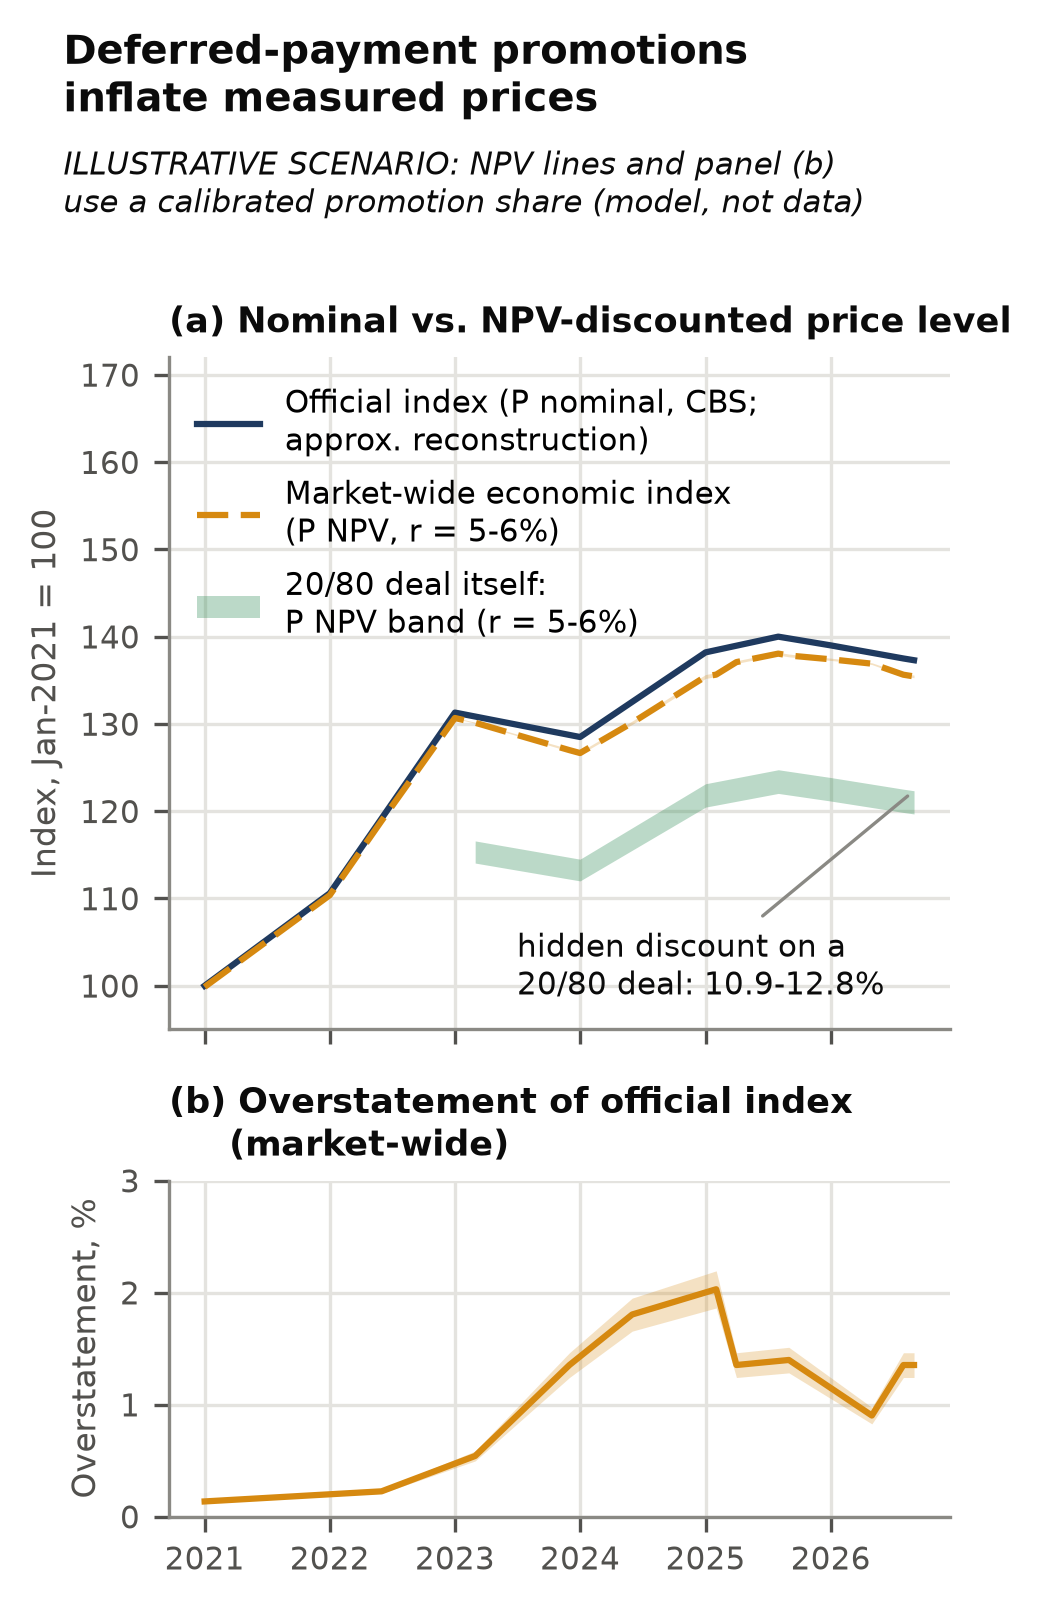
\includegraphics[width=0.55\textwidth]{figures/fig3_npv_price_discount_gap.png}
\caption[מדד המחירים הרשמי לעומת המחיר הכלכלי המהוון (\en{NPV})]{מדד מחירי הדירות הרשמי לעומת המחיר הכלכלי המהוון (\en{NPV}) בשיעור היוון של \en{5\%–6\%}. רמות המדד הרשמי הן שחזור משוער; קווי ה־\en{NPV} הם תרחיש להמחשה}
\label{fig:npv-gap}
\end{figure}

\paragraph{סימולציית מונטה קרלו של יחס ההחזר.}\label{subsec:ch5-mc} כדי לאמוד כמה קונים יחצו את ספי ה־\en{PTI} של הוראה \en{329} (סעיף~\ref{sec:ch3-baseline}) ביום המסירה, נדגמו \en{10,000} משקי בית. מחיר הדירה וההכנסה נדגמו מהתפלגות לוג־נורמלית דו־ממדית עם מתאם של \en{0.55}, שיעור המימון מהתפלגות \en{Beta(9,4)} שנקטעה ב־\pct{75}, תקופת ההלוואה \en{25} או \en{30} שנה, ונוסף זעזוע הכנסה אקראי עם סטיית תקן של \pct{5} בין החתימה למסירה. אותן דגימות שימשו לשלושה תרחישי ריבית משכנתה (\pct{4.00}, \pct{5.25} ו־\pct{6.50}).

\paragraph{רשת מבחני הקיצון ליזם ולבנק.}\label{subsec:ch5-stress} רשת מבחני הקיצון בוחנת פרויקט מייצג של \en{200} דירות (להמחשה), שמהן \pct{60} נמכרו מראש, בשני ממדים: ירידת מחירים של \en{0\%–20\%} ועיכוב במסירה של \en{0–24} חודשים (\en{81} תאים). ההכנסות מנורמלות ל־$R=1$, העלויות הן \en{0.83}, והאשראי הבנקאי $L$ הוא \pct{70} מהעלויות. כאשר הירידה במחיר עולה על \pct{5}, חלק מקוני המבצעים מבטלים, והדירות נמכרות מחדש בהנחה נוספת של \pct{5}. העיכוב מוסיף ארבעה רכיבי עלות: התייקרות בנייה, ריבית על האשראי, המשך סבסוד ריבית הבלון, ופיצוי לקונים לפי חוק המכר \cite{salelaw1974} (דמי שכירות מוכפלים, בהנחת \nis{7,500} לחודש). שני מדדי התוצאה הם:

\begin{align}
\mathrm{DSCR} &= \frac{\mathrm{Rev}(p,m) - C - O(m) + L}{L}, \label{eq:ch5-dscr}\\
\mathrm{Coverage} &= \frac{(1-p)\,R\,(1-h) - O(m)}{L + G}, \label{eq:ch5-coverage}
\end{align}

כאשר $O(m)$ עלויות העיכוב, $h$ קיצוץ ערך הבטוחה ו־$G$ ערבויות חוק המכר שהבנק נתן לקונים (\pct{30} מהתמורה ששולמה מראש). $\mathrm{DSCR}<1$ פירושו שהיזם אינו יכול לפרוע את האשראי מתזרים המסירה, ו־$\mathrm{Coverage}<100\%$ פירושו שהבטוחה אינה מכסה את חשיפת הבנק.

\paragraph{מודל שחיקת ההון העצמי רובד \en{1}.}\label{subsec:ch5-cet1} כשל של רוכש אינו כשל של בנק. הרוכש הנכשל מחזיר את הדירה ליזם, הדירה נמכרת מחדש בהנחה וכרית הביטחון של הפרויקט נשחקת; הבנק מפסיד רק כשהיא מתאפסת. הכרית נמדדת ב\term{כושר ספיגה}{Absorption Capacity}: הירידה המרבית במחירי המכירה שאינה גורמת לבנק הפסד \cite{boi_survey2025}. עבור שיעור כשל רוכשים $\delta$, ירידת מחיר $q$ ועיכוב $m$, השחיקה במונחי מחיר של המלאי שטרם נמכר היא:

\begin{equation}
x=q+\frac{\pi\varphi\,\delta\,[1-(1-q)(1-c)]+O(m)}{1-\pi}
\label{eq:ch5-erosion}
\end{equation}

כאשר $\pi=0.6$ שיעור המכירה המוקדמת, $\varphi=0.45$ חלק המבצעים ו־$c$ הנחת המכירה מחדש. חלק החשיפה הנכשל הוא $\zeta F(x)$, כאשר $F$ ההתפלגות המצטברת של כושר הספיגה לפי אשראי: \pct{8} מתחת ל־\pct{30} ו־\pct{33} מתחת ל־\pct{40} \cite{boi_survey2025}, ויתר הנקודות מדוחות לאומי והפועלים \cite{leumi_q3_2026,hapoalim_q3_2026}, שהגדרותיהם שונות (סעיף~\ref{sec:ch5-limitations}). ההפסד ושחיקת יחס ההון של בנק $b$ הם:

\begin{align}
N_b &= \max\{0,\; \ell\,(sD_b+gG_b)-sP_b\}, \quad \ell_A = \zeta F(x)\,[1-(1-q)(1-k)], \label{eq:ch5-loss}\\
\Delta\mathrm{CET1}_b &= \frac{N_b(1-t)}{\mathrm{RWA}_b}, \quad \ell_B = \zeta\,\frac{1-\pi}{\lambda}\int_0^{x}F(a)\,da, \label{eq:ch5-cet1}
\end{align}

כאשר $s$ חלק הדיור באשראי, $k$ עלות המימוש, $t$ שיעור המס ו־$\lambda=0.761$ החשיפה ליחידת הכנסה. גרסה $A$ שמרנית בירידות המחיר שנבחנו (לפרויקט שנכשל לא נותרה כרית, וירידת המחיר פועלת פעמיים); גרסה $B$ מודדת רק את עומק הגירעון וללא מכירת חירום. ערבות שמומשה נוספת לחשיפה מול הדירה שחזרה, ולכן אינה נספרת פעמיים. נכסי הסיכון קבועים ורווחי הבנק אינם מקוזזים. לפי תיעוד הצוות, הכלל נקבע לפני ההרצה: תנאי ה־\pct{10} מתקיים אם שתי הגרסאות עומדות בו בתרחיש (כשל \pct{25}, ירידה \pct{20}, \en{24} חודשים), אינו מתקיים אם שתיהן חורגות, ואם הן חלוקות התוצאה תלויה בשיטה ואינה מכריעה. הבחינה לפני מס; \mbox{\en{REQ-H3-01}} אינה קובעת בסיס מס, ולכן מדווחת גם התוצאה אחרי מס. חישוב ידני ללאומי ($A$) מחזיר את תוצאת הקוד (\en{194} נ״ב). טבלה~\ref{tab:ch5-banks} מציגה את נתוני הבנקים.

\begin{table}[!htb]
\centering
\caption[נתוני חמש הקבוצות הבנקאיות]{נתוני המודל לחמש הקבוצות הבנקאיות, \en{30.9.2026} (מיליארדי \en{₪}; יחסים באחוזים)}
\label{tab:ch5-banks}
\footnotesize
\begin{tabularx}{\tabmaxwidth}{>{\raggedleft\arraybackslash}p{3.1cm} C C C C C C C}
\toprule
\hd{קבוצה} & \hd{\en{CET1}} & \hd{מזערי} & \hd{\en{RWA}} & \hd{הון} & \hd{$D$} & \hd{$G$} & \hd{$P$} \\
\midrule
לאומי \cite{leumi_q3_2026} & \en{11.38} & \en{10.23} & \en{623.4} & \en{71.4} & \en{149.3} & \en{48.0} & \en{3.4} \\
הפועלים \cite{hapoalim_q3_2026} & \en{11.62} & \en{10.24} & \en{580.6} & \en{67.5} & \en{116.1} & \en{31.5} & \en{2.6} \\
מזרחי־טפחות \cite{mizrahi_q3_2026} & \en{10.10} & \en{9.60} & \en{368.1} & \en{36.7} & \en{54.4} & \en{18.3} & \en{0.7} \\
דיסקונט \cite{discount_q3_2026} & \en{10.32} & \en{9.21} & \en{347.1} & \en{35.1} & \en{56.5} & \en{17.5} & \en{1.3} \\
הבינלאומי \cite{fibi_q3_2026} & \en{10.28} & \en{9.24} & \en{143.3} & \en{14.5} & \en{24.5} & \en{3.0} & \en{0.5} \\
\bottomrule
\end{tabularx}

\smallskip
$D$ חובות בינוי ונדל״ן בישראל; $G$ ערבויות לרוכשי דירות (נומינלי, לפני ביטוח משנה); $P$ הפרשה להפסדי אשראי
\end{table}

\section{כיול הפרמטרים ומגבלות}
\label{sec:ch5-calibration}

טבלה~\ref{tab:ch5-calibration} מרכזת את הפרמטרים המכוילים; רק מרכיבי $s$ ושיעור המס הם נתונים ממקור.

\begin{table}[!htb]
\centering
\caption[פרמטרים מכוילים (להמחשה)]{פרמטרים מכוילים (להמחשה), ערכיהם והנימוק לבחירתם}
\label{tab:ch5-calibration}
\footnotesize
\begin{tabularx}{\tabmaxwidth}{>{\raggedleft\arraybackslash}p{4.0cm} >{\centering\arraybackslash}p{2.7cm} R}
\toprule
\hd{פרמטר} & \hd{ערך} & \hd{נימוק} \\
\midrule
שיעור היוון $r$ & \en{5\%–6\%} & פריים ועוד מרווח \\
דחיית תשלום $T$, חלק נדחה $d$ & \en{3} שנים, \en{0.8} & בנייה טיפוסית, \en{20/80} \\
משקל דירות חדשות $w_{\mathrm{new}}$ & \en{0.38} & סדר גודל של חלקן בעסקאות \\
שיעור מבצעים $s(t)$ & \en{3\%–45\%} & \pct{30} באוגוסט \en{2026} (חמישה אזורים, מסירה משנה ומעלה) \cite{mof_review_2026_08} \\
מחיר והכנסה חציוניים & \nis{2.4M}, \nis{26,000} & סדר גודל \\
ריביות משכנתה & \pct{4.0}, \pct{5.25}, \pct{6.5} & ריבית \pct{3.25} ועוד מרווחים \\
שולי רווח יזם, אשראי לעלות & \pct{17}, \pct{70} & ליווי סגור, סדר גודל \\
ריבית אשראי יזם & \pct{7.25} & פריים \pct{4.75} ועוד \pct{2.5} \\
קוני מבצעים במכירה מוקדמת & \pct{45} & שיעור המבצעים בשיאו \\
קיצוץ ערך בטוחה $h$ & \pct{10} & מכירה כפויה \\
חלק הדיור $s$ & \pct{40.9} & \en{150/367}: פרויקטים וקרקע למגורים \cite{boi_survey2025} \\
מימוש ערבויות $g$, העברה $\zeta$ & \en{1}, \en{1} & שמרני; נבחן \en{0–0.5}, \en{0.25–0.5} \\
עלויות $c$, $k$; מס $t$ & \pct{5}, \pct{5}; \pct{34.75} & להמחשה; סטטוטורי \cite{discount_q3_2026} \\
כשל רוכשים, ירידת מחיר & \en{15\%–25\%} & \en{PTI} מעל \pct{50} באיור~\ref{fig:pti-mc} (\en{16\%–27\%}); תרחיש \\
\bottomrule
\end{tabularx}
\end{table}

\label{sec:ch5-limitations}שלוש מגבלות עיקריות: (\en{1}) הפרויקט ברשת מייצג ואינו מדגם, ופיזור מאזני היזמים רחב יותר; (\en{2}) עוגני \en{2021–2023} במלאי ובעסקאות לא אומתו; (\en{3}) המודלים אינם כוללים השפעות חוזרות (ירידת מחירים, ביטולים, גידול במלאי וירידה נוספת), ולכן תוצאות הרשת עשויות להמעיט בסיכון. מודל ההון מאחד נתוני כושר ספיגה משני מועדים, מייחס אותם גם לקרקע ומחיל חלק דיור אחיד על כל הבנקים; הוא אינו מבחן קיצון רשמי. גם ההגדרות שונות: לאומי מודד את כושר הספיגה מול מחירי המלאי, והפועלים (\pct{53} מהאשראי בשלוש מהנקודות) מול שווי הנכס כגמור; המודל מחיל את הגדרת לאומי, והשנייה הופכת את התוצאה (סעיף~\ref{sec:ch6-cet1}).
